\documentclass{xetexCV}
%\usepackage[newsec,reorder]{cvsplitbib}
%\usepackage[newsec,reorder,export]{splitbib}
\usepackage[sorting=ydnt,maxnames=18,firstinits=true]{biblatex}
\usepackage{xstring}
\usepackage{url}
\usepackage{fontspec}
%\usepackage{hyperref}

%\setmainfont[Ligatures={Common}, Numbers={OldStyle}]{Warnock Pro}
\setmainfont{Cambria}
\setsansfont{Calibri}
%\setsansfont{Frutiger LT Std}

\addbibresource{bib/pcmember.bib}
\addbibresource{bib/varrodan.bib}

\newcommand{\makeauthorbold}[1]{%
  \DeclareNameFormat{author}{%
    \ifthenelse{\value{listcount}=1}
    {%
      {\expandafter\ifstrequal\expandafter{\namepartfamily}{#1}{\mkbibbold{\namepartfamily\addcomma\addspace \namepartgiveni}}{\namepartfamily\addcomma\addspace \namepartgiveni}}
      %
    }{\ifnumless{\value{listcount}}{\value{liststop}}
        {\expandafter\ifstrequal\expandafter{\namepartfamily}{#1}{\mkbibbold{\addcomma\addspace \namepartfamily\addcomma\addspace \namepartgiveni}}{\addcomma\addspace \namepartfamily\addcomma\addspace \namepartgiveni}}
        {\expandafter\ifstrequal\expandafter{\namepartfamily}{#1}{\mkbibbold{\addcomma\addspace \namepartfamily\addcomma\addspace \namepartgiveni\addcomma\isdot}}{\addcomma\addspace \namepartfamily\addcomma\addspace \namepartgiveni\addcomma\isdot}}%
      }
    \ifthenelse{\value{listcount}<\value{liststop}}
    {\addcomma\space}
  }
}

\makeauthorbold{Varr{ó}}

 
%\renewcommand{\refname}{List of Publications}
%\setcounter{SBresetdepth}{2}
%\renewcommand{\refname}{}

%----------------------------- Service to Community ---------------------
%\begin{category}{Service to Scientific Community} 
%\begin{category}[CH]{Program Co-Chair}
%  \SBentries{sle2016-chair,icmt2014-chair,fase2013-chair,amt2012-chair,agtive2011-chair,grabats2010-chair,gtvmt2006-chair,grabats2006-chair}
%\end{category}
%
%\begin{category}[SC]{Steering Committee Member}
%  \SBentries{etaps2008-sc,etaps2013-sc}
%\end{category}
%
%\begin{category}[LO]{General Chair / Local Organizing Chair }
%  \SBentries{staf2013-chair,models2012-chair,sensus2009-lo,etaps2008-lo,models2007-chair,edcc2005-lo}
%\end{category}
%
%\begin{category}[JR]{Journals}
%  \SBentries{sosym,scp,ieee-tse,acm-tosem,sttt,ause}
%\end{category}
%
%\begin{category}[DS]{Opponent (External PhD reviewer)}
%  \SBentries{Ciccozzi,Kalauz,Hildebrandt,Zombori,Guta,Siikarla,Lundkvist,Meszaros,Gergely,Vidacs,Hettel,Sipos,Lukacsy,Hajdara}
%\end{category}
%
%\begin{category}[CH]{Chair of Doctoral Committee}
%  \SBentries{Vajk}
%\end{category}
%
%
%\end{category}
 
%----------------------------- PC Membership ---------------------

%\begin{category}{Program Committee Membership} 
%
%\begin{category}[SE]{Software Engineering}
%  \SBentries{icse2018-pc,fase2017-pc,%
%ase2016-pc,models2016-pc,ecmfa2016-pc,%
%ase2015-pc,models2015-pc,sle2015-pc,fase2015-pc,%
%ase2014-pc,models2014-pc,fase2014-pc,%
%  models2013-pc,ecmfa2013-pc,%
%  models2012-pc,ase2012-pc,ase2012tools-pc,icse2012tools-pc,%
%  fase2012-pc,csmr2012-pc,ecmfa2012-pc,icmt2012-pc,%
%  ase2011-pc,ase2011tools-pc%
%  models2011-pc,fase2011-pc,icmt2011-pc,ecmfa2011-pc,sofsem2011-pc,%
%  mbsdi2011-pc,melo2011-pc,%
%  models2010-pc,fase2010-pc,icmt2010-pc,ase2010-pc,modelsedu2010-pc,%
%  models2009-pc,fase2009-pc,icmt2009-pc,ase2009-pc,%
%  models2008-pc,icmt2008-pc,aramis2008-pc,%
%  wapl2007-pc,modelsedu2007-pc,modeva2007-pc,atem2007-pc,sac2007-pc,%
%  sac2006-pc,iwmec2006-pc,modeva2006-pc,atem2006-pc,gramot2006-pc,cmt2006-pc,gamma2006-pc,%
%  mtip2005-pc,gramot2005-pc%
%  }
%\end{category}
%
%\begin{category}[VT]{Visual Modeling Techniques and Tools}
%  \SBentries{gam2015-pc,vlhcc2014-pc,vlhcc2013-pc,vlhcc2012-pc,gtvmt2012-pc,%
%  vlhcc2011-pc,gtvmt2011-pc,%
%  gtvmt2010-pc,%
%  gtvmt2009-pc,%
%  gtvmt2008-pc,grabats2008-pc,%
%  gtvmt2007-pc,agtive2007-pc,%
%  fujaba2006-pc,fujaba2005-pc,grabats2004-pc%
%  }
%\end{category}
% 
%\begin{category}[DC]{Dependable Computing}
%  \SBentries{ewdc2011-pc,dsn2009-pc,edcc2006-pc,icdcs2006-pc}
%\end{category}
%
%\begin{category}[FM]{Formal Methods}
%  \SBentries{icgt2014,icgt2012-pc,icgt2012ds-pc,%
%  ictac2011-pc,icgt2010-pc,ictac2010-pc,%
%  fm2009-pc,%
%  icgt2008-pc,pngt2008-pc,%
%  icgt2006-pc,gtvc2006-pc,gtvc2005-pc}
%\end{category}
%
%\begin{category}[ED]{Education}
%	\SBentries{models2010edu-pc,models2007edu-pc}
%\end{category}
%\end{category}

%\nocite{*}
%\SBtitlestyle{bar}
%\SBsubtitlestyle{none}

%\begin{category}{Publications} 
%\begin{category}[B]{Books and Book Chapter (Total: 8)}
%  \SBentries{fmi2004,nagl65-2010,bpel2sal-sensoria-book,sensoria-uml,SENSORIABook:AdvancesInGT,mdegt2005_ggzvvv,caise2011-revised,fmic2005_pv}
%\end{category}
% 
%\begin{category}[J]{Refereed Journals (Total: 21)}
%%  \SBentries{ist2015,scp2015,ause2014,sosym2014-trace,sosym2012-tools,sosym2011-cdt,sosym2011-csp,Bergmann-sttt10,Gilmore-sosym10,Rath-sosym09,sosym2008-mtbe,ijcsse08-kgv,scp-2007,sosym2005_bhtv,hiradas2006-hvv,sosym2005_db,sosym2004_mc,FundInf2003_ghv,pp2003_as,sosym2003_vpm,SCP2002} 
%  \SBentries{SCP2002,sosym2003_vpm,pp2003_as,FundInf2003_ghv,sosym2004_mc,sosym2005_db,hiradas2006-hvv,sosym2005_bhtv,scp-2007,ijcsse08-kgv,sosym2008-mtbe,Rath-sosym09,Bergmann-sttt10,Gilmore-sosym10,sosym2012-tools,sosym2011-cdt,sosym2011-csp,scp2015,ause2014,ist2015,sosym2014-trace} 
%\end{category}
%
%\begin{category}[C]{Peer Reviewed Conference Papers (Total: 48)}
%%  \SBentries{ase2014,models2014-iqd,models2014-stream,sle2014,csmr2014,models2013,models2012,ecmfa2012,icgt2012-ts,icst2012,tools2012,ase2011-dse,ase2011-mtslice,ase2011-tool,vlhcc2011,ecmfa2011,icmt2011,models-2010-incquery,ServiceWave2011,SEFM10:back-ann,Bergmann-icmt08,Horvath-models09,Rath-models09,icgt08-bhrv,Gonczy-mdwe08,icmt08-rbov08,Rath-vlhcc08,agtive07-vhv,isas-2007-kv,sac2007-vb,sac06_vtcl,sac06_plugin,isas2006_kvn,models2006-varro,icgt2006,isas05_bvp,fase2005_eeltvv,vlhcc05_vsv,wicse2004_bhtv,GI2004,icgt2004_rsv,uml2004_meta,esec03_bhtv,uml2003_tool,ASE2002,ICGT2002-GHV02,ICGT2002-SC,UML2002} 
%  \SBentries{UML2002,ASE2002,ICGT2002-GHV02,ICGT2002-SC,%
%esec03_bhtv,uml2003_tool,%
%wicse2004_bhtv,GI2004,icgt2004_rsv,uml2004_meta,%
%isas05_bvp,fase2005_eeltvv,vlhcc05_vsv,%
%sac06_vtcl,sac06_plugin,isas2006_kvn,models2006-varro,icgt2006,%
%agtive07-vhv,isas-2007-kv,sac2007-vb,%
%icgt08-bhrv,Gonczy-mdwe08,icmt08-rbov08,Rath-vlhcc08,%
%Bergmann-icmt09,Horvath-models09,Rath-models09,%
%SEFM10:back-ann,models-2010-incquery,%
%ase2011-dse,ase2011-mtslice,ase2011-tool,vlhcc2011,ecmfa2011,icmt2011,ServiceWave2011,%
%models2012,ecmfa2012,icgt2012-ts,icst2012,tools2012,models2013,%
%ase2014,models2014-iqd,models2014-stream,sle2014,csmr2014} 
%\end{category}
%
%\begin{category}[O]{Other Conference Papers (Total: 3)}
%  \SBentries{dasc2010-hvs,Daboczi-AWSN2013,dasc2014}
%\end{category}
%   
%\begin{category}[W]{Refereed Workshop Papers (Total: 42)}
%%  \SBentries{cmseba2014,mpm2014,oss4mde2014,bigmde2014,bigmde2013,ocl2012,amt2012-query,eceasst2010-guided,eceasst2011-type,SEFM10ToolDemo:back-ann,Bergmann-gtvmt09,Gonczy-safecomp08,gramot08-borvv,gtvc2006-gkv,GT-VMT2007-hvv,efts-2007-kgv,cmt2006,gtvmt06_dpv,wsmate2006,gramot2005_tax,dspd2006_rv,pngt2006-vv,models2006-edu,gramot2005_adapt,gramot2006-vvs,mtip2005,gtvmt04_gsv,grabats2004_vfv,gtvmt04_vv,cbse03_bhtv,DDECS2003_tvp,csduml2003,GRABATS2002,edcc2002_svp,GTVMT2002,FMOODS2002,AGT2002,WTUML01,GRATRA2000,DDECS2000}
%  \SBentries{GRATRA2000,DDECS2000,WTUML01,%
%edcc2002_svp,GTVMT2002,FMOODS2002,AGT2002,GRABATS2002,%
%cbse03_bhtv,DDECS2003_tvp,csduml2003,%
%gtvmt04_gsv,grabats2004_vfv,gtvmt04_vv,%
%gramot2005_adapt,gramot2006-vvs,mtip2005,%
%cmt2006,gtvmt06_dpv,wsmate2006,gramot2005_tax,dspd2006_rv,pngt2006-vv,models2006-edu,gtvc2006-gkv,%
%GT-VMT2007-hvv,efts-2007-kgv,%
%Gonczy-safecomp08,gramot08-borvv,%
%Bergmann-gtvmt09,%
%SEFM10ToolDemo:back-ann,eceasst2010-guided,%
%eceasst2011-type,%
%ocl2012,amt2012-query,%
%Kolovos-bigmde2013,Izso-bigmde2013,%
%bigmde2014,cmseba2014,mpm2014,oss4mde2014,vao2014}
%\end{category}
%
%\begin{category}[I]{Invited Papers (Total: 5)}
%%  \SBentries{csmr2012-invited,models09-edu,agtive07-toolcontest,Wirsing-isola08,easst2006-etv}
%  \SBentries{easst2006-etv,Wirsing-isola08,agtive07-toolcontest,models09-edu,csmr2012-invited}
%\end{category}
%
%\begin{category}[E]{Edited Volumes (Total: 7)}
%%  \SBentries{icmt2014,fase2013,amt2012,agtive2011,grabats2010,icgt2006-grabats,gtvmt2006}
%  \SBentries{gtvmt2006,icgt2006-grabats,grabats2010,agtive2011,amt2012,fase2013,icmt2014}
%\end{category}
%
%\end{category}


  
\cvname{D\'aniel Varr\'o}
%\cvimage{figures/varro.jpg}
\cvimage{figures/VarroD-2015-small.jpg}
%\institution{Contact Address:} 
%\contactaddress{Arany J\'anos u. 77. fszt.1 \\
%Budapest, H-1221, Hungary}
%\phonenumber{+36-30-2438706}
%\email{daniel.varro@gmail.com}

\institution{Contact Address:} 
\contactaddress{3480 Rue University, McConnell Engineering Building \\
Department of Electrical and Computer Engineering \\
McGill University \\
Montreal, QC, Canada, H3A 0E9}
%\phonenumber{+1-514-5831084}
\email{daniel.varro@gmail.com}

%\institution{Contact Address: }
%\contactaddress{Electrical and Computer Engineering Department\\
%McGill University \\
%3480 University Street \\
%Montreal, QC, H3A0E9\\
%Canada}
%\email{daniel.varro@mcgill.ca}

%\contactaddress{Department of Measurement and Information Systems \\
% Budapest University of Technology and Economics \\
%Magyar tud\'osok krt. 2 \\
%Budapest, H-1117 \\
%Hungary}
%\email{varro@mit.bme.hu}
%\website{http://www.inf.mit.bme.hu/en/members/varro}  
%\url{http://www.mit.bme.hu/~varro}

\hyphenpenalty=10000

% Set the Font to Warnock Pro and Frutiger LT Std
%\setmainfont[Ligatures={Common}, Numbers={OldStyle}]{Fontin}
%\setsansfont{Fontin Sans}

\begin{document}
\makecvtitle

\cvsection{Education and Degrees}
Doctor of Science (DSc); \years{2013}Hungarian Academy of Sciences  
%\newline This degree is a formal prerequisite of full professorship in Hungary. \\


Habilitation; \years{2011}Budapest University of Technology and Economics (shortly BME) 

PhD \years{2004}in Software Engineering (official name: Technical Informatics);
BME %Budapest University of Technology and Economics \\

MSc \years{2000}in Software Engineering (official name: Technical Informatics); 
BME %Budapest University of Technology and Economics  

\cvsection{Academic Positions}
Professor \years{2016 - }, Electrical and Computer Engineering (ECE) Department, McGill University

Research Chair \years{2015 - } of MTA-BME Lendulet Research Group on Cyber-Physical Systems \\ Hungarian Academy of Sciences 

Professor, \years{2014 - } Dept. of Measurement and
Inf. Systems, BME  (on leave)

Visiting Professor, \years{2014} Dept. of Computer Science, McGill University, Canada

%Visiting Professor \years{2014}, D\'epartemente d'informatique et de recherche op\'ertionnelle, Universit\'e de Montr\'eal, Canada
Visiting Professor, \years{2014} DIRO, Universit\'e de Montr\'eal, Canada

Associate Professor (tenured), \years{2009 - 2014} Dept. of Measurement and
Inf. Systems, BME 	

Assistant Professor\years{2005 - 2009}, Dept. of Measurement and
Information Systems, BME 

Lecturer\years{2003 - 2005}, Dept. of Measurement and Information
Systems, BME

\cvsection{Research Interests}
Model based software and systems engineering, Cyber-physical systems, \\
Formal methods, Critical embedded systems, Graph based tools and databases
%A draft research statement is available at:
%\url{https://dl.dropboxusercontent.com/u/62723032/LERO/VarroD_ResearchStatement.pdf}
%Application areas: critical embedded systems, service-oriented applications

\cvsection{Publication highlights}
Total number of papers (with DBLP classification): 163 \\
Books and book chapters: 9 \\
Peer reviewed (regular and electronic) journal papers: 46 \\
%Peer reviewed journal papers (incl. peer reviewed electronic journals): 35  (46) \\
%(incl. 10 in Software and Systems Modeling, Springer) \\
Peer reviewed conference (+ workshop) papers: 67 (+33)  \\
%Refereed workshop papers: 31: \\
Number of citations: 6328 (as of August 1st, 2018 by Google Scholar) \\
%Number of citations: 3613 (as of November 30th, 2014 by CIDS 3.0) \\
%(of which in Scopus: 839, in MTMT: 1501) \\ 
%h-index (by CIDS): 31, g-index (by CIDS): 56, h-index (in MTMT): 26,\\
h-index (by Google Scholar): 41 \\
Source: \url{http://scholar.google.pt/citations?user=4Ya6dVoAAAAJ} 
%\url{http://cids.fc.ul.pt/cids_3_0/results.php?acc=3741130101140333046} \\
%\url{https://vm.mtmt.hu/www/index.php?AuthorID=10001355}
%ResearchNet: \url{https://www.researchgate.net/profile/Daniel_Varro/publications}
%\url{http://cids.di.fc.ul.pt/cids_3_0/results.php?acc=19271126111105329059}

\cvsection{Research Visits} 
Universit\'e de Montr\'eal \years{2014} (Prof. Houari Sahraoui) and McGill University (Prof. Hans Vangheluwe),  6 months


TU Berlin, Germany (2x 1 month, with Prof. Hartmut Ehrig, SEGRAVIS Grant)
\years{2004, 2005} 

Univ. Paderborn, Germany \years{2003} (3 months, with Prof. Gregor Engels,
SEGRAVIS) \

SRI International, US (4 months, with Dr. John Rushby) \years{2001} 


\cvsection{Projects and Grants} 


\cvsubsection{Canadian Projects (as PI or co-PI)}
\textbf{NSERC-DG}: \years{2016 - 2021} Model-based Design and Validation Techniques for
Smart and Safe Cyber-Physical Systems (RGPIN-2016-04573), PI, own funding: 230,000 CAD \\
\textbf{NSERC CRD}: \years{2017 - 2022} Digital Multidisciplinary Analysis and Design Optimization Platform for Aeroderivative Gas Turbines, co-PI, total/own funding: 1,177,500 CAD / 235,500 CAD \\
\textbf{McGill Startup Fund}: \years{2016 - 2019} Initial research support: 55,000 CAD \\
\textbf{McGill}: \years{2016 - 2018} 3 small teaching support funds: total around 5,000 CAD \\


\cvsubsection{Collaborative European Projects (as Site Leader or Research
Coordinator at our site)}
\textbf{MONDO}: \years{2013 - 2016} Scalable Modelling and Model Management 
on the Cloud (EU-FP7-ICT-STREP, own funding: 420,000 EUR)  \\
\textbf{E-Freight}: \years{2010 - 2013}European e-Freight Capabilities for
Co-modal Transport (EU-FP7-SST-IP, own funding: 260,000 EUR)  \\
\textbf{SecureChange}: \years{2009 - 2012}Security Engineering for Lifelong
Evolvable Systems (EU-FP7-FET-IP, 231101-2009, own funding: 250,000 EUR)  \\ 
\textbf{DIANA}: \years{2006 - 2010}Distributed, equipment Independent
environment for Advanced avioNic Applications (EU-STREP, FP6-2005-Aero-1, own funding: 410,000 EUR) \\
\textbf{SENSORIA}: \years{2005 - 2010}Software Engineering for Service Oriented
Overlay Computers (FP6 European IP, IST-016004, own funding: 300,000 EUR)  

\cvsubsection{Hungarian National Projects (as PI)}


\textbf{MTA-BME Lend\"ulet} \years{2015-2020} Research Group on Cyber-Physical Systems, 520 000 EUR\\

\textbf{CERTIMOT}: \years{2010-2014}Design and Analysis Techniques for
Certifiable Model Transformations (ERC-HU-09: Starting Grant\footnote{My
Starting Grant proposal went to the final round at EC with a score of 7/8;
%and it was recommended for funding but became out of budget, 
finally it was partially funded by the Hungarian Research Agency}, 370 000 EUR) 


\cvsubsection{Industrial Research Grants and Projects} 

\textbf{TRANS-IMA}: collaborative project with \years{2012-2014}\textbf{Embraer} on
model-driven avionic design tools (funding: 200 000 EUR) \\

Collaborative project with \years{2013-2014}\textbf{Ericsson} on
modeling and verification of statecharts (funding: 20 000 USD)\\

\textbf{IBM Faculty Award}: \years{2007}A framework for the model-driven design
and analysis of standards-compliant IT infrastructure management (by IBM TJ Watson Research Centre,
funding: 20,000 USD)  \\

\textbf{IBM Faculty Award}: \years{2006}Model based deployment of services to
standards-compliant reliable IBM middleware (by IBM TJ Watson,
funding: 10,000 USD)  \\

\textbf{IBM Faculty Award}: \years{2005}Model Transformation Engineering as a
complement to IBM Process Modeling Technologies (by IBM TJ Watson, 
funding: 6,000 USD)  \\

Two collaborative projects with \years{2006-2010}\textbf{Nokia Research Centre}
on high-availability service platforms, and on MDD%model-driven development
techniques (funding: 40 000 EUR)\\

%\textbf{Total own funding}: approx. 2.2 million EUR \\
\textbf{Total acquired funding}: approx. 3.1 million EUR \\
(This excludes funding I secured as a co-founder of IncQuery Labs Ltd, which also exceeds 800K EUR.)

\cvsection{Further Project Participation} 

\cvsubsection{Collaborative Research Projects (as Contributor)}
\textbf{NECSIS}: \years{2014} (An Automotive Partnership Canada project)  \\
\textbf{INDEXYS}: \years{2009-2011}INDustrial EXploitation of the genesYS
cross-domain architecture (ARTEMIS-2008-1-100021)  \\
\textbf{RESIST}: \years{2006-2008}Resilience for Survivability in IST (EU-FP6
Network of Excellence)  \\
\textbf{DECOS}: \years{2004-2007}Dependable Embedded Components and Systems (FP6
European IP) \\
\textbf{SEGRAVIS}: \years{2002-2006}Syntactic and Semantic Integration of
Visual Modelling Techniques (Research Training Network) 

\cvsubsection{National Research Projects (as  Contributor)}

EC-Conforming \years{2005-2006} Certification of Safety Equipments for Hungarian
Railways (GVOP-2004-3.1.1) \\
Operation Research Methods \years{2001-2003} for the Analysis and Verification
of IT Systems (OTKA T038027) \\ 
Framework \years{2000-2002} for the Development and Testing of Dependable,
Safety-Critical Systems (IKTA-00065/2000) \\  
Formal Methods in Informatics (MEH 96/2000) \years{2000-2001} \\
Automated Verification \years{1999-2001} and Validation of UML Models for IT
Systems (OTKA T030804) 

\cvsubsection{National Projects on innovative exploitation of academic
results (as Major Contributor)}

An MDA \years{2005-2007}based product family for service dependability and
optimization (GVOP-2005-3.3.1, in Hungarian)  


\cvsection{Awards} 
%\emph{The 5 award winning papers (or their journal extensions) are included in my application package}

\textbf{Distinguished Reviewer Award} \years{2018} at ICSE 2018: 40th International Conference on Software Engineering

\textbf{EASST Best Paper Award} \years{2018} at ETAPS 2018 conference  

\textbf{Csanád Imreh Award} \years{2017} (by OTDT Hungary): I was the first ever awardee of the prize (awarded in the field of software engineering and computer science for Hungarian researchers below the age of 41) commemorating the Hungarian computer scientist who tragically died in 2017 at the age of 41.  

ACM \years{2016} \textbf{Distinguished Paper Award} (MODELS 2016: The 19th IEEE/ACM International Conference on Model Driven Engineering Languages and Systems) 

IEEE \years{2016} \textbf{10-Year Most Influential Paper Award} \newline (IEEE VL/HCC 2016 for a paper presented at VL/HCC 2005 conference) 

Springer \years{2014} \textbf{10-Year Most Influential Paper Award} \newline (IEEE/ACM MODELS 2014 for a paper presented at UML2004 conference) 

ACM \years{2014}\textbf{Distinguished Paper Award} \newline (IEEE CSMR-WCRE 2014 Software Evolution Week) 

\textbf{STEM Award} \years{2014} by Tempus Foundation \newline for innovative education methods (introducing VCL cloud based labs)

Springer \years{2013} \textbf{Best Paper Award} (MODELS 2013: The 16th IEEE/ACM International Conference on Model Driven 
Engineering Languages and Systems) 

ACM \years{2011}\textbf{Distinguished Paper Award} (ASE 2011: 26th IEEE/ACM International Conference on Automated Software Engineering) 

\textbf{J\'anos Bolyai Scholarship} \years{2010-2013}(Design and Analysis Techniques
for the Certification of Model Transformations): A national
award of the Hungarian Academy of Sciences for young scholars. It can be awarded
at most twice.

\textbf{Distinguished Tutor}: \years{2009} Bi-annual award for the supervision
of MSc students carrying out early research with 3 awardees in Computer
Science biannually. It requires 10 years of successful tutoring (I
became the youngest ever awardee). 

Springer \years{2009}\textbf{Best Paper Award} and ACM \textbf{Distinguished Paper Award} \newline (MODELS
2009: The 12th IEEE/ACM International Conference on Model Driven Engineering Languages and
Systems) 

\textbf{J\'anos Bolyai Scholarship} \years{2005-2008} (Design and Analysis Techniques
for Automated Model Transformations) 

\textbf{J\'anos Kem\'eny Prize } \years{2003}(An annual
award in Hungary for young scholars issued by John von Neumann Computer Society)

\cvsection{Major Open Source Software Projects}

VIATRA \years{2004-} Model Transformation Framework (Founder): \newline
\url{http://www.eclipse.org/viatra} 
EMF-IncQuery: \years{2010-2016} Incremental queries over EMF models (Co-founder) 
%\url{http://www.eclipse.org/incquery/} \\

MASSIF: \years{2014-} Matlab Simulink Integration Framework for Eclipse (Co-founder) \newline 
\url{https://github.com/viatra/massif} 

%Eclipse Committer \years{2005-}(now in Modeling project) 
%\\

%Key contributor to several other research prototypes 
%CheckVML: \years{2002-2004}Model checking for graph transformation systems
%\\

\cvsection{Invited talks}
\emph{Keynote talk}: Automated \years{2017} Graph Model Generation for Smart and Safe Cyber-Physical Systems (Consortium for Software Engineering Research CSER 2017) \\

\emph{Keynote Talk}: \years{2016} Incremental Queries and Transformations: From Concepts to Industrial Applications  (SOFSEM 2016 conference) 

Graph-based  Design and Analysis Tools for Smart and Safe Cyber-Physical Systems (NASA Jet Propulsion Lab) 

Incremental Queries and Reactive Transformations (DSM-TP 2017 Summer School, Montreal, Canada)

Formal Verification and Validation in Domain-Specific Languages (DSM-TP 2017 Summer School, Montreal, Canada)
	
Model-based Tools for Engineering Cyber-Physical Systems (McGill University Professor Talks)

Scalable  Graph-based techniques for smart cyber-physical systems (Papyrus Industrial Consortium)

Models and Queries for Smart and Safe Cyber-Physical Systems (CSCS 2016 Conference, Szeged)

Challenges for Smart and Trustworthy Cyber-Physical Systems (Ericsson University Day 2016 Budapest)

Incremental Model Queries and Transformations (DSM-TP International Summer School; DSM-TP 2016) \\

EMF/Ecore-based DSL engineering \years{2015} (at Dagstuhl Seminar 15062:  Domain-Specific Languages)

EMF-IncQuery: Incremental Evaluation of Model Queries (DSM-TP 2015) 

VIATRA: Advanced Tools by Reactive Transformations (DSM-TP 2015) \\

\emph{Plenary Talk}: Generic and Meta-Transformations \years{2014} (Most Influential Paper Presentation at @MODELS 2014, Valencia, Spain)

Incremental Model Queries over the Cloud (SERENE 2014 Autumn School, Hungary)


EMF-IncQuery: Incremental Evaluation of Model Queries (DSM-TP 2014)


Traceability Challenges in Design Tools for Avionics (DSM-TP 2014) 

Distributed Incremental  Model Queries over the Cloud: Engineering and Deployment Challenges 
(Keynote at CloudMDE 2014 Workshop @MODELS 2014)


Distributed Incremental Model Queries (GT-VMT 2014 Workshop @ETAPS 2014) \\


Validation of Complex Domain-Specific Modeling Languages \years{2013} (at Dagstuhl Seminar 13211 
Automatic Reasoning on Conceptual Schemas)


V\&V Challenges for Models, Queries and Transformations in Design Tools for Avionics (VOLT 2013 Workshop)


Model queries for secure collaborative modeling (EternalS 2013 Workshop) \\

Keynote speaker \years{2012} at 16th European Conference on Software Maintenance
and Reengineering (CSMR 2012, Szeged, Hungary) 

Developing Design Tools for Critical Embedded Systems: A Model Transformation Playground
(at RISC, Hagenberg, Austria) \\

Designing Domain-Specific Languages (at University of Szeged, Hungary)
\years{2010} \\

Model driven \years{2009} development of configuration tables (at Rockwell Collins, US)
Model transformation development (at SENSUS Summer School, HU)
Service deployment by model transformation (at SENSUS Summer School, HU)
\\

Precise model transformations for tool integration (at TU Berlin, Germany)
\years{2008} \\

Model transformation by example (at ISIS, Vanderbilt University, US)
\years{2007} 

Model-Driven Deployment of Services to Standards Compliant Reliable
Middleware (at Dagstuhl Seminar 07061 Autonomous and Adaptive Web Services)
\\

The VIATRA2 model transformation framework (at TU Darmstadt, Germany)
\years{2004} 

Towards Automated Formal Verification of Visual Modeling Languages
by Model Checking (at Dagstuhl Seminar 04101 Language Engineering for Model-Driven
Software Development) \\

Model checking visual modeling languages (at SRI International, US) \years{2003}

\cvsection{Graduate Supervision and Tutoring}

\textbf{PhD students (main supervisor): 10} --- Istv\'an R\'ath (defended: 2011), \'Akos Horv\'ath (defended: 2013), G\'abor
Bergmann (defended: 2013), \'Abel Heged\"us (defended: 2014), Zolt\'an Ujhelyi (defended: 2017), 
Benedek Izs\'o (2012-2014), 
G\'abor Sz\'arnyas (PhD candidate, 2014- ACM SRC 1st place at MODELS 2017, ACM SRC 2nd place at SIGMOD 2018), Oszk\'ar Semer\'ath (PhD candidate, 2014-), Csaba Debreceni (PhD candidate, 2014-, ACM SRC 1st place at MODELS 2017), 
Andr\'as Szabolcs Nagy (2015- 2017), 
M\'arton B\'ur (2016- )\\

\textbf{PhD students (as co-tutor): 4}: --- Gergely Varr\'o (2008), Andr\'as Balogh (2010), G\'abor Guta (2012), L\'aszl\'o G\"onczy (to complete in 2018) \\

\textbf{Number of Masters students graduated}: 23 completed + 2 ongoing --- now working for companies like
Google (3 students), Morgan Stanley, Ericsson, ThyssenKruppPresta, PwC, Nokia-Siemens Networks, European Chemical Agency, Trendency, IncQuery Labs, Lufthansa Systems, Siemens, National Instruments \\

\textbf{Tutoring MSc students on a national-level scientific competition}: 23
scientific reports; 3x 1st prize (on national level), 3x 3rd prize (on national
level), 12x 1st prize (on faculty level), %8x second prize (on faculty level)) 
Distinguished Tutor (2009) (youngest ever awardee; requires 10 years of
highly successful tutoring) \\

\cvsection{Teaching}
\cvsubsection{Taught Courses at McGill University (Instructor and course co-developer)}

Introduction to Software Engineer (undergraduate, 75-90 students, 2017 Winter, 2018 Winter)

Model based engineering of cyber-physical systems (this is the new course name - graduate, 18 students, 2018 Winter)

%\begin{figure}
%\centering
%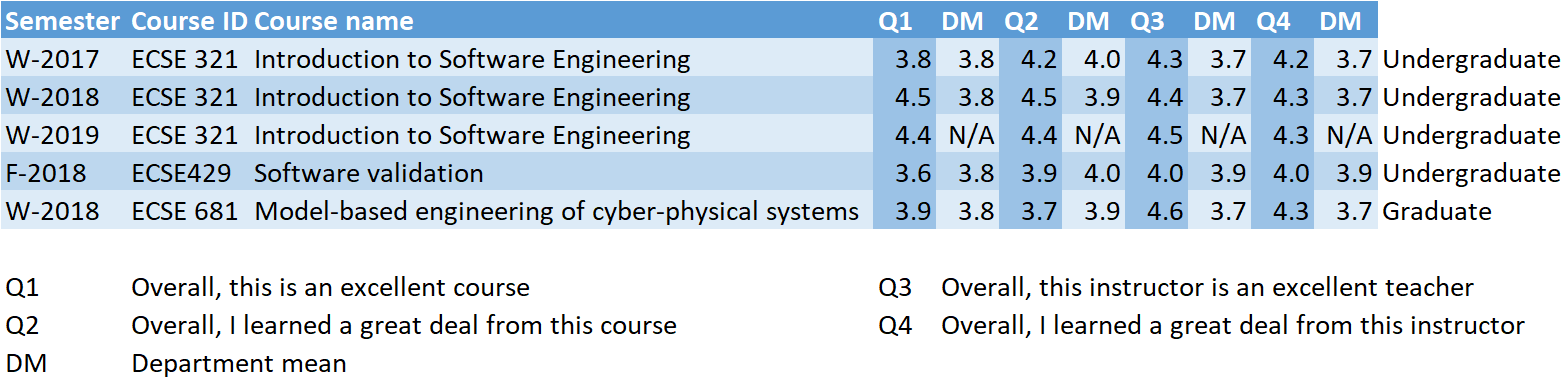
\includegraphics[width=.9\textwidth]{figures/TeachingEval}
%\caption{Results of teaching evaluation at McGill University}
%\end{figure}

\cvsubsection{Taught Courses at BME (Lecturer and course co-developer)}

Model driven system development (2010-, MSc, 15-25 students)

Model driven software development (2010-2014, MSc, 10-20 students)

UML-based modeling and analysis (2002 - 2008, MSc, 70-80 students / year)

Open development frameworks (2005 - 2008, MSc, 10-20 students)

Foundations of model-driven development (2005- , PhD, 5-10 students)

(All these courses were taught for students of software engineering specialized in dependable systems)

\cvsubsection{Supervised Courses}

Systems engineering (2016- , BSc, 60-80 students)

System integration (2010- , MSc, 10-20 students)

Eclipse-based based development and integration (2010- , MSc, 10 students) 

Eclipse technologies (2009- , BSc, 10-20 students) 

\cvsubsection{Participating as Lecturer}

Formal methods (2001 - 2006, BSc, 300-450 students)

\cvsubsection{Teaching Assistant}
 
Formal languages (1999 - 2001, BSc, 20-30 students)

Fault tolerant systems lab (200 - 2001, BSc, 30 students)

\cvsection{Membership in Professional Societies and Committees}
Informatics Committee of Hungarian Academy of Sciences (elected member, 3 times)  \years{2011-} \\
Informatics Doctoral School, BME (core member)  \years{2014-} \\
Informatics Doctoral School, University of Szeged (external member)  \years{2014-} \\
John von Neumann Computer Society (vice-president) \years{2009-2015} \\
Member of IEEE Computer Society \years{2006-}

\cvsection{Industry and Entrepreneurship} 
Co-founder of IncQuery Labs Ltd. (Co-founder and Strategic advisor) \years{2013-}  \\
Co-founder of OptXware Ltd. (Vice-President of Research and Development) \years{2006-2014} \\

\cvsection{Spoken Languages}
Hungarian (mother tongue) \\ 
English (fluent) \\ 
French (intermediate, B2/C1)

%\newpage

\cvsection{Services to the Scientific Community}
%\cvsubsection{Program Co-Chair}

\begin{refsection}
\newrefcontext[labelprefix=CH]
\nocite{sle2016-chair,icmt2014-chair,fase2013-chair,amt2012-chair,agtive2011-chair,grabats2010-chair,gtvmt2006-chair,grabats2006-chair}
\printbibliography[title=Program Co-Chair]
\end{refsection}

\begin{refsection}
\newrefcontext[labelprefix=SC]
\nocite{etaps2008-sc,etaps2013-sc}
\printbibliography[title=Steering Committee Member]
\end{refsection}

\begin{refsection}
\newrefcontext[labelprefix=LO]
\nocite{icse2019post-chair,staf16ws-chair,staf2015ds-chair,staf2013-chair,models2012-chair,sensus2009-lo,etaps2008-lo,models2007-chair,edcc2005-lo}
\printbibliography[title=Chair of Organizing Committees]
\end{refsection}

\begin{refsection}
\newrefcontext[labelprefix=DS]
\nocite{Haussler,Oakes,AlBayati,Beyhl,GasconSamson,DeCarlos,Hegyhati,Vajk,Ciccozzi,Kalauz,Hildebrandt,Zombori,Guta,Siikarla,Lundkvist,Meszaros,Gergely,Vidacs,Hettel,Sipos,Lukacsy,Hajdara}
\printbibliography[title=Participation in PhD Defense Committees]
\end{refsection}

\cvsection{Program Committee Membership}

\begin{refsection}
\newrefcontext[labelprefix=SE]
  \nocite{icse2019-pc,icse2018-pc,fase2018-pc,icmt2018-pc,ecmfa2018-pc,models2018-pc,securemde2018-pc,%
models2017-pc,fase2017-pc,icmt2017-pc,ase2017tools-pc,mise2017-pc,%
ase2016-pc,models2016-pc,ecmfa2016-pc,models2016ds-pc,icmt2016-pc,%
ase2015-pc,models2015-pc,sle2015-pc,fase2015-pc,%
ase2014-pc,models2014-pc,fase2014-pc,%
  models2013-pc,ecmfa2013-pc,%
  models2012-pc,ase2012-pc,ase2012tools-pc,icse2012tools-pc,%
  fase2012-pc,csmr2012-pc,ecmfa2012-pc,icmt2012-pc,%
  ase2011-pc,ase2011tools-pc%
  models2011-pc,fase2011-pc,icmt2011-pc,ecmfa2011-pc,sofsem2011-pc,%
  mbsdi2011-pc,melo2011-pc,%
  models2010-pc,fase2010-pc,icmt2010-pc,ase2010-pc,modelsedu2010-pc,%
  models2009-pc,fase2009-pc,icmt2009-pc,ase2009-pc,%
  models2008-pc,icmt2008-pc,aramis2008-pc,%
  wapl2007-pc,modelsedu2007-pc,modeva2007-pc,atem2007-pc,sac2007-pc,%
  sac2006-pc,iwmec2006-pc,modeva2006-pc,atem2006-pc,gramot2006-pc,cmt2006-pc,gamma2006-pc,%
  mtip2005-pc,gramot2005-pc%
  }
\printbibliography[title=Software Engineering]
\end{refsection}

\begin{refsection}
\newrefcontext[labelprefix=VT]
  \nocite{gam2015-pc,vlhcc2014-pc,vlhcc2013-pc,vlhcc2012-pc,gtvmt2012-pc,%
  vlhcc2011-pc,gtvmt2011-pc,%
  gtvmt2010-pc,%
  gtvmt2009-pc,%
  gtvmt2008-pc,grabats2008-pc,%
  gtvmt2007-pc,agtive2007-pc,%
  fujaba2006-pc,fujaba2005-pc,grabats2004-pc%
  }
\printbibliography[title=Visual Modeling Techniques and Tools]
\end{refsection}

\begin{refsection}
\newrefcontext[labelprefix=FM]
  \nocite{facs2018-pc,fmmdd2016-pc,icgt2014,icgt2012-pc,icgt2012ds-pc,%
  ictac2011-pc,icgt2010-pc,ictac2010-pc,%
  fm2009-pc,%
  icgt2008-pc,pngt2008-pc,%
  icgt2006-pc,gtvc2006-pc,gtvc2005-pc}
\printbibliography[title=Formal Methods]
\end{refsection}


\begin{refsection}
\newrefcontext[labelprefix=DC]
  \nocite{ewdc2011-pc,dsn2009-pc,edcc2006-pc,icdcs2006-pc}
\printbibliography[title=Dependable Computing]
\end{refsection}

\begin{refsection}
\newrefcontext[labelprefix=ED]
\nocite{models2010edu-pc,models2007edu-pc}
\printbibliography[title=Education]
\end{refsection}

\begin{refsection}
\newrefcontext[labelprefix=JR]
\nocite{sosym,scp,ieee-tse,jss,ieee-sw,acm-tosem,sttt,ause}
\printbibliography[title=Journals]
\end{refsection}

\begin{refsection}
\newrefcontext[labelprefix=IJ]
\nocite{cost,nwo,nserc,fct,fwf,mta,simi,york,stellenbosch,udem}
\printbibliography[title=International Juries and Evaluation]
\end{refsection}

\cvsection{Publications of D\'aniel Varr\'o}


\begin{refsection}
\newrefcontext[labelprefix=B]
  \nocite{fmi2004,nagl65-2010,bpel2sal-sensoria-book,sensoria-uml,SENSORIABook:AdvancesInGT,mdegt2005_ggzvvv,caise2011-revised,fmic2005_pv,fmhe2018}
\printbibliography[title=Books and Book Chapter (Total: 9)]
\end{refsection}


\begin{refsection}
\newrefcontext[labelprefix=J]
  \nocite{SCP2002,GRABATS2002j,GTVMT2003j,sosym2003_vpm,pp2003_as,FundInf2003_ghv,%
sosym2004_mc,gtvmt2004-gsv-j,gtvmt2004-vv-j,grabats2004-vfv-j,%
sosym2005_db,gramot2005-j,gramot2005-tax-j,%
sosym2005_bhtv,pngt2006-vv,gramot2006-j,hiradas2006-hvv,%
scp-2007,GT-VMT2007-hvv,gtvc2006-gkv,gtvmt2006-dpv-j,%
ijcsse08-kgv,Gonczy-safecert08,sosym2008-mtbe,%
Rath-sosym09,Bergmann-gtvmt09,%
Bergmann-sttt10,Gilmore-sosym10,eceasst2010-guided,eceasst2011-type,%
sosym2012-tools,sosym2011-cdt,sosym2011-csp,scp2015,ause2015,ist2015,sosym2016-trace,sosym2017-dsl,sosym2018-cep,sosym2016-viatra-invited,sosym2017-mondo,sosym2017-tb,act2017,sosym2018-mt,ieeesw2018} 
\printbibliography[title=Refereed Journals incl. Electronic Journals (Total: 44)]
\end{refsection}
 
\begin{refsection}
\newrefcontext[labelprefix=C]
  \nocite{UML2002,ASE2002,ICGT2002-GHV02,ICGT2002-SC,%
esec03_bhtv,uml2003_tool,%
wicse2004_bhtv,GI2004,icgt2004_rsv,uml2004_meta,%
isas05_bvp,fase2005_eeltvv,vlhcc05_vsv,%
sac06_vtcl,sac06_plugin,isas2006_kvn,models2006-varro,icgt2006,%
agtive07-vhv,isas-2007-kv,sac2007-vb,%
icgt08-bhrv,Gonczy-mdwe08,icmt08-rbov08,Rath-vlhcc08,%
Bergmann-icmt09,Horvath-models09,Rath-models09,%
SEFM10:back-ann,models-2010-incquery,%
ase2011-dse,ase2011-mtslice,ase2011-tool,vlhcc2011,ecmfa2011,icmt2011,ServiceWave2011,%
models2012,ecmfa2012,icgt2012-ts,icst2012,tools2012,models2013,%
ase2014,models2014-iqd,models2014-stream,sle2014,csmr2014,%
icmt2015,icgt2015,%
fase2016-solver,fase2016-merge,icgt2016,MODELS2016-access,MODELS2016-bx,MODELS2016-metrics,%
esec-fse2017,models2017,adbis2017,icmt2017,%
icse2018-solver,icse2018-gamma,fase2018-diverse,fase2018-cps,models2018,vlhcc2018,nfm2018} 
\printbibliography[title=Peer Reviewed Conference Papers (Total: 67)]
\end{refsection}

\begin{refsection}
\newrefcontext[labelprefix=O]
  \nocite{dasc2010-hvs,Daboczi-AWSN2013,dasc2014}
\printbibliography[title=Other Conference Papers (Total: 3)]
\end{refsection}


\begin{refsection}
\newrefcontext[labelprefix=W]
  \nocite{GRATRA2000,DDECS2000,WTUML01,%
edcc2002_svp,FMOODS2002,AGT2002,%GRABATS2002,GTVMT2002,
cbse03_bhtv,DDECS2003_tvp,csduml2003,%
%grabats2004_vfv,gtvmt04_vv,gtvmt04_gsv,
mtip2005,%gramot2005_tax,gramot2005_adapt,gramot2006-vvs,
cmt2006,wsmate2006,dspd2006_rv,models2006-edu,%pngt2006-vv,gtvc2006-gkv,gtvmt06_dpv,
efts-2007-kgv,%GT-VMT2007-hvv,
gramot08-borvv,%Gonczy-safecert08,
%Bergmann-gtvmt09,
SEFM10ToolDemo:back-ann,%eceasst2010-guided,
ocl2012,amt2012-query,%
Kolovos-bigmde2013,Izso-bigmde2013,%
bigmde2014,cmseba2014,mpm2014,oss4mde2014,vao2014,%
staf2015-project,ttc2015,gemoc2015,%
BX2016,STAF-proj-2016,commitmde2016,%
commitmde2017}
\printbibliography[title=Refereed Workshop Papers (Total: 33)]
\end{refsection}
  

\begin{refsection}
\newrefcontext[labelprefix=I]
  \nocite{easst2006-etv,Wirsing-isola08,agtive07-toolcontest,models09-edu,csmr2012-invited,sofsem2016-invited,pame2015}
\printbibliography[title=Invited Papers (Total: 7)]
\end{refsection}

\begin{refsection}
\newrefcontext[labelprefix=E]
  \nocite{gtvmt2006,icgt2006-grabats,grabats2010,agtive2011,amt2012,fase2013,icmt2014,staf2015-ds,sle2016,staf2016-ws}
\printbibliography[title=Edited Volumes (Total: 10)]
\end{refsection}



% Automatically Generated Bibliography

%\cvsection{Family and Hobbies}
%married and proud father of two sons (6 and 4 years old) \\
%
%futsal (indoor soccer); \years{1997-2003, 2010-} goalkeeper in 1st and 2nd
%league of the Hungarian National Futsal Championship \\
%
%music (singing in choirs, and participating in concerts for children)

%\nocite{*}\bibliographystyle{ieeetr}
%\bibliography{bib/pcmember,bib/varrodan}

\end{document}